\chapter{Epidemics and higher-order spreading}
\label{ch:epidemics}

In this chapter we apply the two before it. An epidemic is
a percolation problem; a population that mixes both inside households and
across a wider contact network is a chygraph with three layers and nothing
else; and the household reproduction number of mathematical epidemiology drops
out of Chapter~\ref{ch:percolation}'s threshold tensor with no epidemiology
supplied.

Sections~\ref{sec:sirperc}--\ref{sec:rstar} are exposition of solved work.
Section~\ref{sec:groupcontagion} is the step past it. If catching
the disease requires \emph{several} infected members of a group rather than
one, the problem leaves the class of Chapter~\ref{ch:percolation} altogether ---
and it leaves it in exactly the way Sec.~\ref{sec:breakdown} said such a thing
would have to. That is where an outbreak can become explosive, and the rule
behind it is Chapter~\ref{ch:ising}'s unanimity interaction, stated for a
spreading process rather than for a Hamiltonian.

\section{An epidemic is a percolation problem}
\label{sec:sirperc}
\index{SIR model|textbf}
\index{epidemic|textbf}
\index{transmissibility}

Take the SIR model: individuals are susceptible, become infected, and recover
to immunity. An infected individual transmits along each of their contacts at
rate $\beta$ and remains infectious for a period $\tau$. Whether a given
contact ever carries the infection is then settled by a single number,
\begin{equation}
  T=1-e^{-\beta\tau},
  \label{eq:transmissibility}
\end{equation}
the \emph{transmissibility}, and --- this is the observation of
\citet{newman2002} --- if $\tau$ is the same for everyone, the outcome on each
contact is decided independently of every other. So one may decide all of them
in advance, before the epidemic runs: keep each contact with probability $T$,
discard it otherwise. The set of people an initial case eventually infects is
the connected component of that individual in the resulting graph.

Bond percolation, in other words, with $T$ in the role of the bond occupation
probability. The final size of a major outbreak is the giant component
fraction, and the epidemic threshold is the percolation threshold. Everything
in Chapters~\ref{ch:percolation} and~\ref{ch:giant} therefore applies without
translation, which is a large return on one paragraph of argument.

\paragraph{What the mapping does not give.} Two limitations, and the second is
often overlooked.

It gives the final size and not the time course. Percolation is a statement
about which individuals are ultimately reached, and the epidemic curve --- when
the peak arrives, how high it is --- is not in it.

And it needs the infectious period to be the same for everyone. If $\tau$ is
random, the transmissions out of one individual are no longer independent: they
share that individual's period, so a long-lived case infects many contacts and
a short-lived one few. The threshold survives, because it depends on a mean.
What does not survive is the identification of two quantities that coincide in
undirected percolation: the probability that a randomly chosen seed starts a
major outbreak, and the fraction of the population such an outbreak reaches.
Correlated transmission makes the percolation problem directed, the two split
apart, and the standard calculation returns the size
\citep{kenah2007,miller2007}. Quoting it as an outbreak probability is a real
error, not a refinement.

Both limitations are inherited from percolation and neither has anything to do
with higher-order structure. Within them, the rest of this chapter is
Chapter~\ref{ch:percolation} with epidemiological vocabulary.

\section{Two levels of mixing}
\label{sec:twolevels}
\index{households|textbf}
\index{two levels of mixing|textbf}

Real populations do not mix uniformly. People live in households, where contact
is intense and everyone meets everyone; they also meet a scattering of people
outside, at work, on transport, at school. \citet{ball1997,ball2010} built
the standard model of this --- \emph{two levels
of mixing} --- and it has an epidemiological literature of its own.

It is a chygraph with three layers, and drawing it is most of the work
(Fig.~\ref{fig:households}):
\begin{itemize}
\item layer $0$: individuals, as atoms;
\item layer $1$: households, as complexes whose intra-complex graph is the
      complete graph on their members;
\item layer $2$: global contacts, as complexes holding two individuals.
\end{itemize}

Two features of the mapping carry all of the content, and both are statements
one would make in words about households anyway.

\paragraph{A household is a sink, not a route.} Every individual belongs to
exactly one household. Hence $\kappa_{01}\equiv1$, so
\begin{equation}
  \Phi^{0}_{1}(x)=x,
  \qquad
  \bar\Phi^{0}_{1}=1,
  \qquad
  \ave{\kbar}_{01}=0.
  \label{eq:sink}
\end{equation}
An individual reached \emph{from} their household has no second household to
pass through. Households on their own therefore never percolate, whatever
$p_{H}$: $\theta=-1$ for every value of it. The global layer is what connects
one household to the next, and the household layer amplifies what arrives. The
calculation is the one already done in Sec.~\ref{sec:structurebystructure};
that single zero is the only difference in the input.

\paragraph{A household outbreak is a percolated clique.} A Reed--Frost epidemic
in a closed group of $n$ individuals, each pair transmitting with probability
$p_{H}$, is bond percolation on the complete graph $K_{n}$. So the
within-household final size distribution --- the classical object of the
epidemiological literature \citep{ball1986} --- is nothing other than the
intra-complex generating function $\bar G^{1}_{0}$ of
Sec.~\ref{sec:ensembles}. The two are the same calculation, done once.

\begin{figure}[t]
\centering
\begin{adjustbox}{max width=0.95\linewidth}
\begin{tikzpicture}
% Three layers, drawn as an inclusion diagram: households (layer 1) above the
% individuals (layer 0) they contain, global contacts (layer 2) below.
\node[cpx,minimum size=3.4mm] (H1) at (0,1.45) {};
\node[cpx,minimum size=3.4mm] (H2) at (3.2,1.45) {};
\node[atm] (a1) at (-0.85,0.40) {}; \node[atm] (a2) at (0,0.40) {};
\node[atm] (a3) at (0.85,0.40) {};
\node[atm] (b1) at (2.35,0.40) {}; \node[atm] (b2) at (3.2,0.40) {};
\node[atm] (b3) at (4.05,0.40) {};
\draw[inc] (H1)--(a1) (H1)--(a2) (H1)--(a3)
           (H2)--(b1) (H2)--(b2) (H2)--(b3);
\node[cpxc,minimum size=2.6mm] (G1) at (1.60,-0.65) {};
\node[cpxc,minimum size=2.6mm] (G2) at (3.62,-0.65) {};
\node[cpxc,minimum size=2.6mm] (G3) at (-0.42,-0.65) {};
\draw[inc] (G1)--(a3) (G1)--(b1) (G2)--(b2) (G2)--(b3) (G3)--(a1) (G3)--(a2);
\node[lb,anchor=west,align=left] at (4.45,1.45) {households:\\ interior $\bar G^{1}_{0}$};
\node[lb,anchor=west,align=left] at (4.45,0.40) {individuals};
\node[lb,anchor=west,align=left] at (4.45,-0.65) {contacts:\\ transmit with $T$};
% the sink: exactly one line leaves each individual upwards
\node[lb,anchor=east,align=right] at (-1.25,0.95) {one line up\\ per individual};
\draw[msg] (-1.20,0.80) to[out=-20,in=150] (-0.98,0.55);
\end{tikzpicture}
\end{adjustbox}
\caption{\textbf{Two levels of mixing is a three-layer chygraph.} Individuals
are atoms; a household is a complex whose interior is the complete graph on its
members; a global contact is a complex holding two individuals. Each individual
lies in exactly one household, Eq.~\eqref{eq:sink}, so an infection arriving in
a household spreads inside it and stops --- the household layer amplifies but
does not conduct. Conduction is the business of the global layer, and the two
enter the threshold in different ways because of it.}
\label{fig:households}
\end{figure}

\begin{calculation}{the final size of a household outbreak}
Let $C_{j}(p)$ be the probability that the random graph $G(j,p)$ is connected,
which satisfies the standard recursion obtained by conditioning on the
component of a fixed vertex,
\[
  C_{j}(p)=1-\sum_{i=1}^{j-1}\binom{j-1}{i-1}C_{i}(p)\,(1-p)^{i(j-i)},
  \qquad C_{1}=1.
\]
The percolation cluster of a given vertex of $K_{n}$ then has size $j$ with
probability
\begin{equation}
  P_{n}(j)=\binom{n-1}{j-1}\,C_{j}(p_{H})\,(1-p_{H})^{\,j(n-j)}:
  \label{eq:Kn}
\end{equation}
choose the other $j-1$ members, require their induced subgraph to be connected,
and require every one of the $j(n-j)$ links to the outside to be absent. For an
epidemic, $j$ is the final size of the household outbreak including the index
case, so
\[
  \bar G^{1}_{0}(y)=\sum_{j}P_{n}(j)\,y^{\,j-1}
\]
counts the \emph{additional} cases, which is what an inclusion into the
household layer transmits. Mixing over households means mixing over the
\emph{size-biased} size distribution $nP(n)/\ave{n}$, because a household is
reached through one of its members and a large household has more of them.

At $n=3$ Eq.~\eqref{eq:Kn} returns
\[
  \begin{aligned}
    \bar G^{1}_{0}(y)&=(3p_{H}^{2}-2p_{H}^{3})y^{2}+2p_{H}(1-p_{H})^{2}y\\
    &\quad+(1-p_{H})^{3}+p_{H}(1-p_{H})^{2},
  \end{aligned}
\]
which is Eq.~\eqref{eq:tripgf} --- the bond-percolated triangle of
Sec.~\ref{sec:structurebystructure}, term for term, with $p_{H}$ where $q$
stood. A three-person household and an over-represented triangle are the same
object with different names, and the mean number of additional cases is
$\mu_{H}=\bar s_{\triangle}(p_{H})=2p_{H}(1+p_{H}-p_{H}^{2})$.
\end{calculation}

What a user of the software has to supply is a dictionary of household sizes.
Everything else --- the size-biasing, the connectivity recursion, the filling of
$\Phi^{0}_{1}(x)=x$ into the table --- follows from the mapping. The
epidemiology enters through one table entry and nothing else.

\section{The household reproduction number}
\label{sec:rstar}
\index{reproduction number|textbf}

Substituting into the threshold tensor of Sec.~\ref{sec:threshold}, with a
Poisson global contact network of mean degree $\ave{k}$ and global
transmissibility $T$, gives
\begin{equation}
  \theta+1=T\bigl[\ave{\bar k}+\mu_{H}\ave{k}\bigr]\equiv R^{\ast},
  \label{eq:Rstar}
\end{equation}
with $\mu_{H}=\bar G^{1\prime}_{0}(1)$ the mean number of \emph{additional}
household members infected.

Equation~\eqref{eq:Rstar} is the household reproduction number of
\citet{ball1997}. It has a plain reading, and the reading is the same
branching argument that has run through the book since
Sec.~\ref{sec:percolation-intro}. A household reached by one global infection
ends up containing $1+\mu_{H}$ cases. The index case makes $T\ave{\bar k}$
further global infections, having used one contact to arrive; each of the
$\mu_{H}$ secondary cases makes $T\ave{k}$, having used none. An outbreak grows
when the total exceeds one.

What has and has not happened here. The epidemiological literature derives $R^{\ast}$ by constructing a branching
process of households and computing its mean offspring number, which is a
purpose-built argument. Here it is a substitution into a tensor that knows
nothing about disease, and the derivation is the same one that produced
Molloy--Reed and the hypergraph threshold in
Sec.~\ref{sec:structurebystructure}. That is the claim about labour that
Chapter~\ref{ch:percolation} opened with, made in a setting where the
purpose-built argument is genuinely well known.

\paragraph{What the branching argument does not give.} $R^{\ast}$ locates the
threshold and stops. The final size of a major outbreak does not follow from
it, and neither does the rate at which that size grows once the threshold is
passed --- the critical amplitude of Sec.~\ref{sec:amplitude}. Both come out of
the same chygraph without further input (Fig.~\ref{fig:householdfig}), and
Table~\ref{tab:households} does both for households of size three on a
Poisson global network with $\ave{k}=2$.
\begin{table}[t]
\centering\small
\begin{tabular}{lccc}
\hline\hline
 & $p_{H}=0$ & $p_{H}=1/2$ & $p_{H}=1$\\
\hline
$\mu_{H}$      & $0$      & $1.25$   & $2$\\
$T_{c}$        & $0.5000$ & $0.2222$ & $0.1667$\\
$B$            & $4.000$  & $5.478$  & $6.667$\\
$S$ at $T=1$   & $0.7968$ & $0.9560$ & $0.9975$\\
\hline\hline
\end{tabular}
\caption{\textbf{Households lower the threshold and steepen the approach to it.} Households of size three on a Poisson global network with $\ave{k}=2$, at three within-household transmission probabilities. $\mu_{H}$ is the mean number of further household infections, $B$ the critical amplitude of Sec.~\ref{sec:amplitude} and $S$ the final size. The $p_{H}=0$ column reduces to bond percolation on a Poisson graph. Generated by \code{figs/epidemics.py}.}
\label{tab:households}
\end{table}
Households do two separable things. They lower the threshold, by a factor of three here. And they steepen the
approach to it: $B$ rises from $4$ to $6.667$, so just above threshold the
outbreak is not merely more likely but larger. The first fact is $R^{\ast}$'s;
the second is not, and it needs one more order of moments.

The $p_{H}=0$ column is the check one wants. With no within-household
transmission the household layer transmits nothing, the chygraph reduces to
bond percolation on a Poisson graph, $T_{c}=1/\ave{k}=1/2$, and $B=4p$ at $p=1$
--- the first row of Table~\ref{tab:amplitudes}, reached down a completely
different code path.

\begin{figure}[t]
\centering
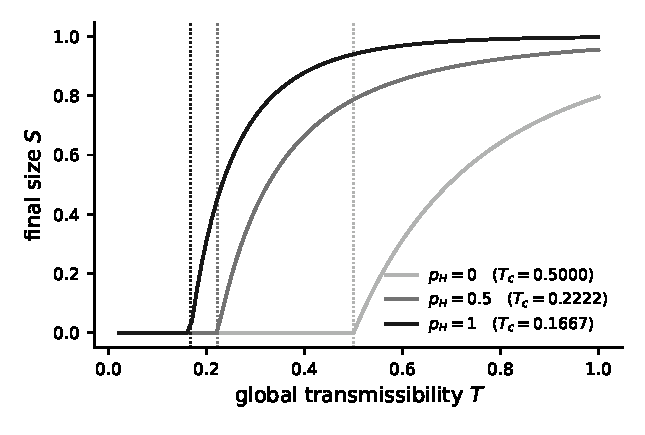
\includegraphics[width=0.9\linewidth]{figs/fig-households.pdf}
\caption{\textbf{Two levels of mixing.} Final size of an SIR epidemic against
the global transmissibility $T$, for households of size three on a Poisson
global contact network with $\ave{k}=2$, at three values of the within-household
transmission probability $p_{H}$. Dotted lines are $R^{\ast}=1$,
Eq.~\eqref{eq:Rstar}. At $p_{H}=0$ the household layer is inert and the curve is
ordinary bond percolation on a Poisson graph. Generated by
\code{figs/epidemics.py}.}
\label{fig:householdfig}
\end{figure}

\paragraph{Loosening the sink.} Equation~\eqref{eq:sink} was the only
epidemiological input, and letting $\Phi^{0}_{1}$ be a genuine degree
distribution instead of the constant $1$ --- individuals belonging to several
groups rather than one --- turns the same chygraph into a \emph{network of
cliques}. That covers SIR with clique-type-dependent transmission, and at
$p_{H}=1$ the connected components of bipartite projections
\citep{fujiki2024proj}. With all cliques of size two it reduces to ordinary bond
percolation and with all of size three to the triangle layer of
Sec.~\ref{sec:structurebystructure} --- two independent code paths that agree.
One dictionary entry separates a household model from a clique network, which
is the sense in which none of this is a family of models.

\section{Contagion inside a group}
\label{sec:groupcontagion}
\index{threshold contagion|textbf}
\index{spinodal}

Everything so far has assumed that one infected member of a group is enough:
the disease enters a household through a single case and spreads by pairwise
contact inside it. Much of what people mean by \emph{higher-order} spreading is
the denial of that assumption. A rumour, a behaviour, a decision to vaccinate
may need reinforcement --- two of three housemates, not one
\citep{watts2002,iacopini2019,stonge2021}. Call it a threshold rule: a group
transmits to a member only when at least $r$ of the others are already
infected.

This looks like a small change and it is not, though the damage is narrower than
it first appears. Chapter~\ref{ch:statmech}'s two steps carry the rule without
modification. What does not carry over is the linear apparatus built on top of
them.

\paragraph{The recursion still closes on one number.} Let $\pi$ be the
probability that a member reached along an inclusion is infected by everything
else attached to it. On a tree the other $c-1$ members of a complex are
independent given $\pi$, so the interior sum of Eq.~\eqref{eq:emitted} is a
binomial tail: a complex of cardinality $c$ fires onto the member entered by
exactly when at least $r$ of the others are infected,
\begin{equation}
  \tau_{c,r}(\pi)=T_{c}\sum_{m\ge r}\binom{c-1}{m}\pi^{m}(1-\pi)^{c-1-m},
  \label{eq:threshtau}
\end{equation}
and the up step is the same product over inclusions as
Eq.~\eqref{eq:Qminus}, with the same bracket: a member reached through layer $m$
escapes only if every one of its other complexes fails to fire, the arriving
inclusion discounted from layer $m$ alone, so
\begin{equation}
  \begin{aligned}
    \pi^{m}&=1-\prod_{l}\bigl[\bar\Phi^{0}_{l}\bigr]_{l=m}
             \bigl(1-\tau_{c_{l},r_{l}}(\pi^{l})\bigr),\\
    \rho&=1-\prod_{l}\Phi^{0}_{l}
          \bigl(1-\tau_{c_{l},r_{l}}(\pi^{l})\bigr),
  \end{aligned}
  \label{eq:threshmap}
\end{equation}
with $\rho$ the infected fraction. This is the two-step recursion of
Sec.~\ref{sec:twosteps} with a threshold interior substituted for a
percolating one, and it carries an arbitrary chy-degree distribution and an
arbitrary mixture of cardinalities and thresholds.

\paragraph{What is lost is the linearisation.} Differentiate
Eq.~\eqref{eq:threshtau} at $\pi=0$. For $r=1$ it gives $T_{c}(c-1)$, the
intra-complex factor of Chapter~\ref{ch:percolation}. For $r\ge2$ it gives
\emph{zero}: $\tau_{c,r}(\pi)\sim\pi^{r}$, so a layer with $r\ge2$ contributes
nothing to the Jacobian of Eq.~\eqref{eq:threshmap} at the trivial fixed point,
whatever its chy-degree. The consequence is visible without any calculation.
With $r\ge2$ a single infected seed cannot activate any group, so it infects
nobody, so $\pi=0$ --- nothing connected to anything --- is not merely a fixed
point but a \emph{stable} one, at every parameter value.
Section~\ref{sec:breakdown} named this exclusion when it arose for
interdependent networks: the transition, if there is one, happens by a
saddle-node bifurcation while the trivial fixed point is still stable, so
$\Lambda=0$ does not locate it, and the threshold tensor of
Sec.~\ref{sec:threshold} --- which is that Jacobian --- reports only the
pairwise layer.

Section~\ref{sec:breakdown}'s proof that group structure alone gives continuous
transitions is untouched by this, and the two are easily confused. That proof
needs the intra-complex function to be a generating function in the
\emph{failure} variable, where all derivatives are non-negative; a threshold
rule is not one, since in $Q=1-\pi$ the failure probability $1-\pi^{r}$ of a
group carries a negative coefficient. So: within the percolation class every
group interaction contributes non-negatively to the curvature $C$ and the onset
is continuous; a threshold rule is outside that class, while remaining inside
the recursion.

\paragraph{The simplest case.} Take a population with two kinds of connection:
Poisson-many pairwise contacts, mean $\ave{k}_{|}$, each transmitting with
probability $T$; and Poisson-many three-member groups, mean
$\ave{k}_{\triangle}$, each transmitting to a member with probability
$T_{\triangle}$ but only when \emph{both} others are infected. Write
\begin{equation}
  \beta_{1}=T\ave{k}_{|},
  \qquad
  \beta_{2}=T_{\triangle}\ave{k}_{\triangle}.
\end{equation}
A Poisson layer is its own excess, $\bar\Phi(x)=\Phi(x)=e^{\ave{k}(x-1)}$, so
$\pi$ and $\rho$ coincide; $\tau_{2,1}=T\rho$ and $\tau_{3,2}=T_{\triangle}\rho^{2}$;
and Eq.~\eqref{eq:threshmap} collapses to
\begin{equation}
  \rho=1-e^{-\beta_{1}\rho-\beta_{2}\rho^{2}}.
  \label{eq:contagion}
\end{equation}
The $\rho^{2}$ is the higher-order physics --- two infected others
required, hence the square --- and everything below is a consequence of it.

\begin{calculation}{where the onset stops being continuous}
Expand the right-hand side of Eq.~\eqref{eq:contagion} about $\rho=0$:
\[
  \rho=\beta_{1}\rho
      +\Bigl(\beta_{2}-\tfrac{\beta_{1}^{2}}{2}\Bigr)\rho^{2}
      +\Bigl(\tfrac{\beta_{1}^{3}}{6}-\beta_{1}\beta_{2}\Bigr)\rho^{3}
      +O(\rho^{4}).
\]
The linear term gives the invasion threshold $\beta_{1}=1$, which involves
$\beta_{2}$ not at all: a seed cannot use the groups, so the groups cannot help
it invade. Setting $\beta_{1}=1$ leaves quadratic coefficient
$\beta_{2}-\tfrac12$ and cubic coefficient $\tfrac16-\beta_{2}$.

When $\beta_{2}<\tfrac12$ the quadratic coefficient is negative, the outbreak
branch leaves the threshold upwards with $\rho\propto(\beta_{1}-1)$, and the
transition is continuous with $\beta=1$ as in Sec.~\ref{sec:amplitude}. When
$\beta_{2}>\tfrac12$ it is positive: the branch leaves \emph{backwards}, exists
below $\beta_{1}=1$, and the transition is discontinuous, with a fold at some
$\beta_{1}<1$. The two are separated by a tricritical point at
\begin{equation}
  \beta_{2}=\tfrac12,
  \label{eq:tricritical}
\end{equation}
where the quadratic term vanishes and the cubic one takes over, giving
$\rho\simeq\sqrt{3(\beta_{1}-1)}$ and the exponent $\beta=\tfrac12$ instead of
$1$. Solving Eq.~\eqref{eq:contagion} numerically at $\beta_{1}-1=10^{-2}$,
$10^{-3}$, $10^{-4}$ gives $\rho/\sqrt{3(\beta_{1}-1)}=0.937$, $0.980$,
$0.994$.

There is no root-finding anywhere in this. Solving Eq.~\eqref{eq:contagion} for
$\beta_{1}$ instead of for $\rho$,
\[
  \beta_{1}(\rho)=\frac{-\ln(1-\rho)-\beta_{2}\rho^{2}}{\rho},
\]
parametrises the whole curve, unstable branch included, and the fold is the
minimum of that function.
\end{calculation}

Figure~\ref{fig:contagion} is the calculation drawn. One dial, $\beta_{2}$,
carries the onset from continuous through tricritical to discontinuous, and at
$\beta_{2}=2$ the fold sits at $\beta_{1}=0.3145$ with $\rho=0.6628$: an
established outbreak survives down to a third of the coupling at which one could
have started. The jump at the invasion threshold is from nothing to
$\rho=0.930$.

\begin{figure}[b]
\centering
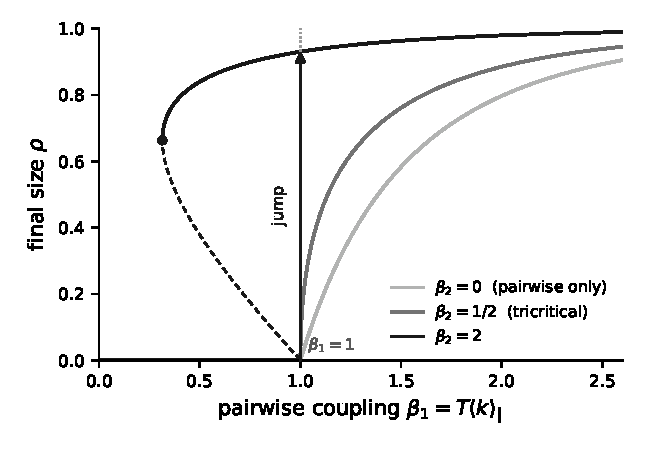
\includegraphics[width=0.9\linewidth]{figs/fig-contagion.pdf}
\caption{\textbf{One dial from continuous to explosive.} Final size against the
pairwise coupling $\beta_{1}$ for Eq.~\eqref{eq:contagion}, at three strengths
$\beta_{2}$ of a group interaction that transmits only when both other members
are infected. Solid lines are stable branches, dashed the unstable one, the
circle the fold. The invasion threshold is $\beta_{1}=1$ whatever $\beta_{2}$;
what $\beta_{2}$ changes is whether the outbreak grows out of it or jumps.
Eq.~\eqref{eq:tricritical} places the boundary at $\beta_{2}=1/2$. Generated by
\code{figs/epidemics.py}.}
\label{fig:contagion}
\end{figure}

Push the dial to the end --- no pairwise route at all, $\beta_{1}=0$ --- and the
invasion threshold disappears rather than moving. No seed can ever start
anything, at any $\beta_{2}$. Yet an outbreak, once present, sustains itself for
all $\beta_{2}>2.4554$, at which point $\rho$ jumps to $0.7153$. A population
with only reinforced transmission cannot be invaded and can be saturated, which
is a statement no threshold calculation would produce, and one a public-health
argument can use.

\paragraph{The equilibrium version of the same thing.} A group that acts only
when all its members agree is Chapter~\ref{ch:ising}'s unanimity interaction:
the simplicial Ising model of \citet{son2026}, whose hyperedges lower the
energy only on their two unanimous configurations. There too the transition is
continuous at small cardinality and discontinuous above a tricritical one, there
too the linear instability of the disordered state is a spinodal rather than the
transition, and there too quoting it as the transition is wrong by ten to fifty
per cent. Chapter~\ref{ch:ising} does that calculation properly, with free
energies. It is the same physics, and the difficulty is the one this section has
already met: a rule that needs several participants at once leaves no linear
instability to locate the transition with.

\section{What higher-order structure does to an outbreak}
\label{sec:epidemics-lessons}

Four things, none of which needs the algebra.

\emph{Groups amplify what reaches them, and it is the amplification that is
counted.} A household does not conduct --- an infection cannot pass through one
household to another, Eq.~\eqref{eq:sink} --- and yet it raises the reproduction
number by a factor of three here, because $\mu_{H}$ multiplies the number of
onward global infections. Conduction and amplification are separate services and
the threshold tensor keeps them in separate entries.

\emph{The amplification saturates.} $\mu_{H}\le n-1$: a household cannot infect
more people than it holds. This is the ``more per branch, fewer branches''
observation of Sec.~\ref{sec:helporhurt} in its most concrete form, and it is
why the fixed-degree and fixed-link-count comparisons of that section come out
with opposite signs.

\emph{Say what is held fixed.} Sec.~\ref{sec:rstar}'s table holds the global
network fixed and adds within-household transmission on top of it, and on that
comparison households help the epidemic a great deal. Hold instead the
\emph{contact budget} fixed --- four contacts per person either way, as
size-three households on a Poisson global network of mean two, against no
households and a Poisson network of mean four, with the same transmissibility
everywhere --- and the sign reverses. The threshold \emph{rises}, from
$T_{c}=0.2500$ to $0.2929$, and at $T=0.3$ the outbreak reaches $5.6\%$ of the
population with households against $31.4\%$ without. Household contacts are
spent repeatedly on the same three people. This is the running thread of
Chapters~\ref{ch:data}, \ref{ch:percolation} and~\ref{ch:giant} appearing once
more, and here it has a public-health reading: whether structure helps or hurts
depends on whether the structured contacts are additional to the rest or taken
out of them.

\emph{Percolation-type spread is always continuous; reinforced spread need not
be.} If one infected contact suffices, the outbreak grows out of its
threshold smoothly, and Sec.~\ref{sec:breakdown} proves this cannot be
otherwise for anything in the percolation class. If several are required, the
outbreak can appear at full size or not at all, cannot be started by a single
seed, and persists below the coupling at which it could have begun. Which r\'egime
a real spreading process is in is an empirical question, and the two make
completely different predictions about what an intervention does.

\section{Checks}
\label{sec:epidemics-checks}

\checkhead{Known results}
Equation~\eqref{eq:Rstar} is verified symbolically against
$T[\ave{\bar k}+\mu_{H}\ave{k}]$ for several household size distributions,
including mixtures of sizes, with $\mu_{H}$ computed independently from the
connectivity recursion; that expression is \citeauthor{ball1997}'s household
reproduction number. Equation~\eqref{eq:Kn} at $n=3$ is checked term by term
against the bond-percolated triangle of Sec.~\ref{sec:structurebystructure},
Eq.~\eqref{eq:tripgf}, symbolically in $p_{H}$. The $p_{H}=0$ column of
Sec.~\ref{sec:rstar}'s table reproduces bond percolation on a Poisson graph,
$T_{c}=1/\ave{k}$ and $B=4$, along a code path that has never heard of
households.

\checkhead{New results}
The critical amplitude for households, and the threshold-rule recursion
Eq.~\eqref{eq:threshmap} with its tricritical point, have no published
counterpart. The amplitudes are obtained by numerical eigenvectors on the full
index set, independently of the symbolic route of Sec.~\ref{sec:amplitude}.
Equation~\eqref{eq:threshmap} is checked against forward simulation of the
contagion on random chygraphs at $n=4\times10^{5}$, over eight combinations of
$\beta_{1}$, $\beta_{2}$ and seed fraction, agreeing to $10^{-3}$ or better in
every case. The tricritical condition Eq.~\eqref{eq:tricritical} is checked in
two ways: symbolically, that the quadratic coefficient at $\beta_{1}=1$ is
$\beta_{2}-\tfrac12$; and numerically, that the fold lies below $\beta_{1}=1$
exactly when $\beta_{2}>\tfrac12$. The exponent $\beta=\tfrac12$ at the
tricritical point is confirmed by solving Eq.~\eqref{eq:contagion} at three
decades of $\beta_{1}-1$.

\checkhead{Partial results}
Everything here is a final size and not a time course, and everything assumes
one infectious period for everyone; Sec.~\ref{sec:sirperc} says what breaks when
it is random. Equation~\eqref{eq:threshmap} inherits Chapter~\ref{ch:overlap}'s
limitation unchanged, since a threshold rule is no more forgiving of overlapping
complexes than a percolating one. And it comes without the apparatus that makes
Chapter~\ref{ch:percolation} quick: with $r\ge2$ the threshold tensor reports
only the pairwise layer, so every transition here is found by following the
branch rather than by linearising, and the edges of a coexistence window are
located one at a time.
